%%%%%%%%%%%%%%%%%%%%%%%%%%%%%%%%%%%%%%%%%%%%%%%%%%%%%%%%%%%%%%%%%%% 
%                                                                 %
%                            ROOT FILE                            %
%                                                                 %
%%%%%%%%%%%%%%%%%%%%%%%%%%%%%%%%%%%%%%%%%%%%%%%%%%%%%%%%%%%%%%%%%%% 
 
\documentclass[chap]{thesis}

% Use the first command below if you want captions over 1 line indented. A side
% effect of this is to remove the use of bold for captions. To restore bold,
% also include the second line below.
\usepackage[hang]{caption2}      % to indent subsequent lines of captions
\usepackage{graphicx}
\usepackage{alltt}
\usepackage{verbatim}
\usepackage{listings}
\usepackage{html}
\renewcommand{\captionfont}{\bfseries} % bold caption (needed with caption 
                                       % package; otherwise bold is default)

\begin{document}
%begin{latexonly} 
\lstset{
  language=Java,
  morekeywords={token,self,behavior,join,currentContinuation},
  basicstyle=\small, 
  stringstyle=\ttfamily,
  frame=single,
  aboveskip=0pt,
  belowskip=0pt  
}
%end{latexonly}
%%%%%%%%%%%%%%%%%%%%%%%%%%%%%%%%%%%%%%%%%%%%%%%%%%%%%%%%%%%%%%%%%%% 
%                                                                 %
%                            TITLE PAGE                           %
%               Master's Thesis or Master's Project               %
%                                                                 %
%%%%%%%%%%%%%%%%%%%%%%%%%%%%%%%%%%%%%%%%%%%%%%%%%%%%%%%%%%%%%%%%%%% 

% Supply information for use on title page:    
\thesistitle{\bf The SALSA Programming Language\\ $\salsaversion$  Release Tutorial}        
\author{Carlos A. Varela, Gul Agha, Wei-Jen Wang, \\
Travis Desell, Kaoutar El Maghraoui, Jason LaPorte, \\
Abe Stephens, Robin Toll, and Gregory Haik}        
%begin{latexonly}
\degree{Computer Science}
\thadviser{}
%\projadviser{Galileo} % for a masters project (instead of \thadviser)        
       % if you have 2 advisers you can use \thadviser and \cothadviser       
       % (or \projadviser and \coprojadviser) 
\submitdate{February 2007}        

\copyrightyear{2007}   % if omitted, current year is used.        
%end{latexonly} 
% Print titlepage and other prefatory material:   
\titlepage        
\copyrightpage         %optional           
\tableofcontents        
%\listoftables          %required if there are tables
%\listoffigures         %required if there are figures

   % titlepage material for Master's thesis or project

%%%%%%%%%%%%%%%%%%%%%%%%%%%%%%%%%%%%%%%%%%%%%%%%%%%%%%%%%%%%%%%%%%% 
%                                                                 %
%                            CHAPTER ONE                          %
%                                                                 %
%%%%%%%%%%%%%%%%%%%%%%%%%%%%%%%%%%%%%%%%%%%%%%%%%%%%%%%%%%%%%%%%%%% 
 
\chapter{Introduction}\label{Introduction}

\section{The SALSA Distributed Programming Language}
\label{The SALSA Distributed Programming Language}
With the emergence of Internet and mobile computing, a wide range 
of Internet applications have placed new demands and challenges 
such as openness, portability, ability to adapt quickly to changing 
execution environments, and highly dynamic reconfiguration. Current 
programming languages and systems lack support for dynamic 
reconfiguration of applications, where application entities get
moved to different processing nodes at run-time.

Java has provided a lot of support to dynamic web content through 
applets, network class loading, bytecode verification, security, 
and multi-platform compatibility. Moreover, Java is a good framework 
for distributed Internet programming because of its standardized 
representation of objects and serialization support. 
Some of the important libraries that provide support for Internet 
computing are: {\tt java.rmi} for remote method invocation, 
{\tt java.reflection} for run-time introspection, {\tt java.io} for 
serialization, and {\tt java.net} for sockets, datagrams, and URLs.

SALSA (Simple Actor Language, System and Architecture) 
\cite{varela-agha-salsa-oopsla-2001} is an 
actor-oriented programming language designed and implemented to 
introduce the benefits of the actor model while keeping the advantages 
of object-oriented programming. Abstractions include active objects, 
asynchronous message passing, universal naming, migration, and advanced 
coordination constructs for concurrency. SALSA is pre-processed into 
Java and hence preserves many of Java's useful object oriented concepts- 
mainly, encapsulation, inheritance, and polymorphism. SALSA abstractions 
enable the development of dynamically reconfigurable applications. A SALSA
program consists of universal actors that can ne migrated to distributed 
nodes at run-time.

\section{Structure of the Tutorial}\label{Structure of the Tutorial}
This tutorial covers basic concepts of SALSA and illustrates its concurrency 
and distribution models through several examples. Chapter \ref{Actor-Oriented Programming} introduces the 
actor model and how SALSA supports it. Chapter \ref{Writing Concurrent Programs} introduces concurrent 
programming in SALSA, including token-passing continuations, join 
blocks, and first-class continuations.Chapter \ref{Writing Distributed Programs} discusses SALSA's 
support for distributed computing including asynchronous message sending, 
universal naming, and migration. Chapter \ref{Advanced Concurrency Coordination} introduces several advanced 
coordination constructs and how they can be coded in SALSA. 
Chapter \ref{actorGarbageCollection} defines actor garbage and
explains how automatic actor garbage collection works in SALSA.
Appendix \ref{nameserverop} introduces how to specify name server options and how to run applications
with different system properties. Appendix \ref{DebuggingTips} provides debugging tips for 
SALSA programs. Appendix \ref{LearningSALSAEx} provides brief descriptions of 
SALSA example programs. Appendix \ref{GRAMMAR} lists the SALSA grammar.


%%%%%%%%%%%%%%%%%%%%%%%%%%%%%%%%%%%%%%%%%%%%%%%%%%%%%%%%%%%%%%%%%%% 
%                                                                 %
%                            CHAPTER TWO                          %
%                                                                 %
%%%%%%%%%%%%%%%%%%%%%%%%%%%%%%%%%%%%%%%%%%%%%%%%%%%%%%%%%%%%%%%%%%% 
 
\chapter{Actor-Oriented Programming}\label{Actor-Oriented Programming}
SALSA is an actor-oriented programming language. This chapter starts 
first by giving a brief overview of the actor model. Section 2 
illustrates how SALSA supports the actor model.

\section{The Actor Model}\label{The Actor Model}
Actors \cite{agha-actors-86,hewitt-actors-77} provide a flexible model of concurrency for open 
distributed systems. Actors can be used to model traditional functional, 
procedural, or object oriented systems. Actors are independent, 
concurrent entities that communicate by exchanging messages 
asynchronously. Each actor encapsulates a state and a thread of 
control that manipulates this state. In response to a message, 
an actor may perform one of the following actions (see Figure~\ref{fig1}):
\begin{itemize}
\item Alter its current state, possibly changing its future behavior.
\item Send messages to other actors asynchronously.
\item Create new actors with a specified behavior.
\item Migrate to another computing host.
\end{itemize}

%begin{latexonly} 
\begin{figure}
\vspace{2.0in}
\begin{center}
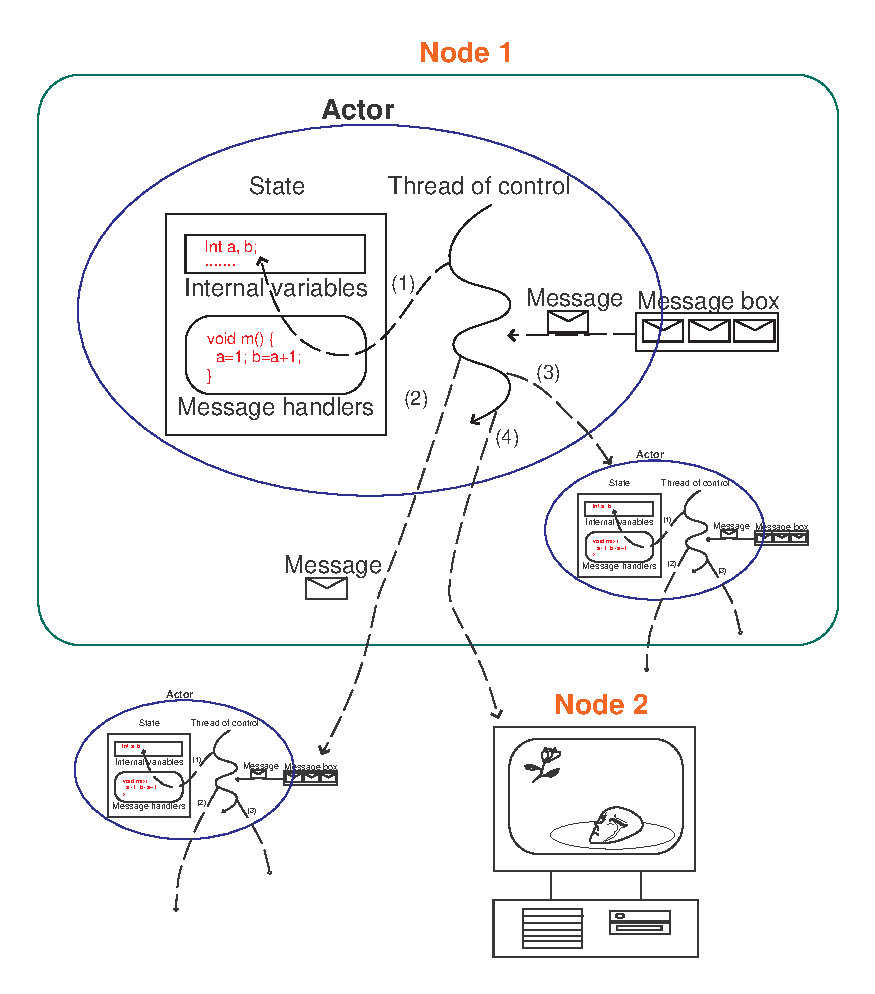
\includegraphics[angle=0,scale=0.75]{fig1.eps}
\caption{Actors are reactive entities.  In response to a message, an
actor can (1) change its internal state, 
(2) send messages to peer actors, 
(3) create new actors, 
and/or (4) migrate to another computing host.}
\label{fig1}
\end{center}
\end{figure}
%end{latexonly} 
\begin{htmlonly}
\begin{figure}
    \htmlimage{thumbnail=0.5}
    \htmlborder{5}
 \includegraphics[width=5in]{img1.png}
\caption{Actors are reactive entities.  In response to a message, an
actor can (1) change its internal state, 
(2) send messages to peer actors, 
(3) create new actors, 
and/or (4) migrate to another computing host.}
\label{fig1}
\end{figure}
\end{htmlonly}

Actors receive messages not necessarily in the same order that they 
were sent. All the received messages are initially buffered in the 
receiving actor's message box before being processed. 
Communication between actors is weakly fair: an actor infinitely 
often ready to receive a message will eventually get it. An actor can 
interact with another actor only if it has a reference to it. Actor 
references are first class entities. They can be communicated in 
messages to allow for arbitrary actor communication topologies. 
Because actors can create arbitrarily new actors, the model supports
unbounded concurrency. Furthermore, because actors only communicate
through asynchronous message passing, in particular because there is
no shared memory, actor systems are highly reconfigurable.

\section{How SALSA Supports the Actor Model}
\label{How SALSA Supports the Actor Model}
SALSA programmers write behaviors which include encapsulated state
and message handlers for actor instances:
\begin{itemize}
\item New actors get created in SALSA by instantiating particular
behaviors (with the {\tt new} keyword). Creating an actor returns
its reference.
\item The message sending operator ({\tt {\textless}-}) is used to send
messages to actors; messages contain a name that refers to the
message handler for the message and optionally a list of arguments.
\item Actors, once created, process incoming messages, one at a time. 
\end{itemize}

\section{Beyond the Actor Model}\label{Beyond the Actor Model}
While SALSA supports the actor model, it goes further in providing
linguistic abstractions for common coordination patterns in concurrent
and distributed applications. For concurrency, it provides token passing
continuations, join blocks, first-class continuations, named
tokens, and message properties. For distribution, it provides universal
naming abstractions, location-transparent remote communication, and
migration support. Furthermore, SALSA provides automatic local and
distributed garbage collection.

 

\chapter{Writing Concurrent Programs}
\label{Writing Concurrent Programs}
This chapter introduces the basic concepts of SALSA
programming, mainly about concurrency coordination. 
Basic knowledge of Java programming is required.

\section{SALSA Language Support for Actor State Modification}
\label{SALSA Language Support for Actor State Modification}
SALSA is a dialect of Java, and it is intended to reuse as many 
features of Java as possible. SALSA actors can contain internal state 
in the form of Java objects or primitive types. However, it is important 
that this internal state must be completely encapsulated, that is, not
shared with other actors. It is also important that the internal state
be serializable. 
\footnote{SALSA, as of version \salsaversion, does not enforce 
state encapsulation and serializability. This discipline needs to be 
followed by programmers, especially for distributed applications.}
   
The following piece of code illustrates how
the internal state is modified, as follows:

%begin{latexonly} 
{\singlespace
\lstinputlisting[]{code/3.3.txt}
}
%end{latexonly} 

\begin{htmlonly}
 \begin{rawhtml} 
  <table border="1" cellpadding="2" cellspacing="0" style="border-collapse: collapse" bordercolor="#111111" id="AutoNumber1">
   <tr><td><pre>
  \end{rawhtml} 
\input{htmlcode/3.3.txt}
 \begin{rawhtml} 
   </pre></td></tr>
  </table>
\end{rawhtml} 
\end{htmlonly} 


\section{Actor Creation}
\label{Actor Creation}
The actor reference is one of the main new primitive 
values of SALSA. There are three approaches to get an 
actor reference: either by actor creation statement, 
the {\tt getReferenceByName()} function, or passed arguments
from messages. This section only concentrates on actor 
creation and reference passing. 

Writing a constructor in SALSA 
programming is similar 
to object construction in Java programming. 
For instance, one can declare the {\tt HelloWorld}
actor as follows:

%begin{latexonly} 
{\singlespace
\lstinputlisting[]{code/3.1.txt}
}
%end{latexonly} 
\begin{htmlonly}
 \begin{rawhtml} 
  <table border="1" cellpadding="2" cellspacing="0" style="border-collapse: collapse" bordercolor="#111111" id="AutoNumber1">
   <tr><td><pre>
  \end{rawhtml} 
\input{htmlcode/3.1.txt}
 \begin{rawhtml} 
   </pre></td></tr>
  </table>
\end{rawhtml} 
\end{htmlonly} 



To create an actor instance and return a reference to 
{\tt myRef}, one can write code as follows:
%begin{latexonly} 
{\singlespace
\lstinputlisting[]{code/3.2.txt}
}
%end{latexonly} 
\begin{htmlonly}
 \begin{rawhtml} 
  <table border="1" cellpadding="2" cellspacing="0" style="border-collapse: collapse" bordercolor="#111111" id="AutoNumber1">
   <tr><td><pre>
  \end{rawhtml} 
\input{htmlcode/3.2.txt}
 \begin{rawhtml} 
   </pre></td></tr>
  </table>
\end{rawhtml} 
\end{htmlonly} 

In SALSA, actor 
references are passed by reference, while object 
variables by value. Objects are passed by value to 
prevent shared memory and preserve encapsulation.

\section{Message Passing}
SALSA uses asynchronous message passing as its primitive form of communication. 
A SALSA\textit{message handler} is similar to a Java method.
Message passing in SALSA is implemented by  
asynchronous message delivery with 
dynamic method invocation. The following example 
shows how an actor sends a message to itself. 
Note that it is not a Java method invocation:
%begin{latexonly} 
{\singlespace
\lstinputlisting[]{code/3.4.txt}
}
%end{latexonly} 
\begin{htmlonly}
 \begin{rawhtml} 
  <table border="1" cellpadding="2" cellspacing="0" style="border-collapse: collapse" bordercolor="#111111" id="AutoNumber1">
   <tr><td><pre>
  \end{rawhtml} 
\input{htmlcode/3.4.txt}
 \begin{rawhtml} 
   </pre></td></tr>
  </table>
\end{rawhtml} 
\end{htmlonly} 


Another type of message passing statement 
requires a target (an actor reference), 
a reserved token {\tt {\textless}-}, 
and a message handler with arguments to be sent. 
For instance, an actor can send a message to 
the standardOutput actor as follows:
%begin{latexonly} 
{\singlespace
\lstinputlisting[]{code/3.5.txt}
}
%end{latexonly}
\begin{htmlonly}
 \begin{rawhtml} 
  <table border="1" cellpadding="2" cellspacing="0" style="border-collapse: collapse" bordercolor="#111111" id="AutoNumber1">
   <tr><td><pre>
  \end{rawhtml} 
\input{htmlcode/3.5.txt}
 \begin{rawhtml} 
   </pre></td></tr>
  </table>
\end{rawhtml} 
\end{htmlonly} 
 
Note that the following expression is illegal 
because it is neither  
a Java method invocation nor a 
message passing expression:
%begin{latexonly} 
{\singlespace
\lstinputlisting[]{code/3.6.txt}
}
%end{latexonly} 
\begin{htmlonly}
 \begin{rawhtml} 
  <table border="1" cellpadding="2" cellspacing="0" style="border-collapse: collapse" bordercolor="#111111" id="AutoNumber1">
   <tr><td><pre>
  \end{rawhtml} 
\input{htmlcode/3.6.txt}
 \begin{rawhtml} 
   </pre></td></tr>
  </table>
\end{rawhtml} 
\end{htmlonly} 

Message Passing in SALSA is by-value 
for objects, and 
by-reference for actors. Any object
passed as an argument is cloned at the moment it 
is sent, and the cloned object is then sent to the target actor.

\section{Coordinating Concurrency}
\label{Coordinating Concurrency}
SALSA provides three approaches to coordinate behaviors of actors: 
\textit{token-passing continuations}, \textit{join blocks}, 
and \textit{first-class continuations}. 

\subsection{Token-Passing Continuations}
\label{Token passing continuations}
Token-passing continuations 
are designed to specify a partial order of message processing.
The token '{\tt @}' is used to group messages 
and assigns the execution order to each of them. 
For instance, the following example 
forces the {\tt standardOutput} actor, a predefined system actor for 
output, to print out "Hello World":
%begin{latexonly} 
{\singlespace
\lstinputlisting[]{code/3.7.txt}
}
%end{latexonly} 
\begin{htmlonly}
 \begin{rawhtml} 
  <table border="1" cellpadding="2" cellspacing="0" style="border-collapse: collapse" bordercolor="#111111" id="AutoNumber1">
   <tr><td><pre>
  \end{rawhtml} 
\input{htmlcode/3.7.txt}
 \begin{rawhtml} 
   </pre></td></tr>
  </table>
\end{rawhtml} 
\end{htmlonly} 

If a programmer uses '{\tt ;}' instead of 
'{\tt @}', SALSA does not guarantee  
that the standardOutput actor will print out "Hello World". It is 
possible to have the result 
"WorldHello ". The following example shows the 
non-deterministic case:

%begin{latexonly} 
{\singlespace
\lstinputlisting[]{code/3.8.txt}
}
%end{latexonly} 
\begin{htmlonly}
 \begin{rawhtml} 
  <table border="1" cellpadding="2" cellspacing="0" style="border-collapse: collapse" bordercolor="#111111" id="AutoNumber1">
   <tr><td><pre>
  \end{rawhtml} 
\input{htmlcode/3.8.txt}
 \begin{rawhtml} 
   </pre></td></tr>
  </table>
\end{rawhtml} 
\end{htmlonly} 

A SALSA message handler can return a value, and 
the value can be accessed through a reserved keyword '{\tt token}', 
specified in one of the arguments of the next grouped message. 
For instance, assuming there exists a user-defined 
message handler, {\tt returnHello()}, which 
returns a string "Hello". The following example 
prints out "Hello" to the standard output:
%begin{latexonly} 
{\singlespace
\lstinputlisting[]{code/3.9.txt}
}
%end{latexonly}
\begin{htmlonly}
 \begin{rawhtml} 
  <table border="1" cellpadding="2" cellspacing="0" style="border-collapse: collapse" bordercolor="#111111" id="AutoNumber1">
   <tr><td><pre>
  \end{rawhtml} 
\input{htmlcode/3.9.txt}
 \begin{rawhtml} 
   </pre></td></tr>
  </table>
\end{rawhtml} 
\end{htmlonly} 
 
Again, assuming another user-defined message handler 
{\tt combineStrings()}
accepts two input Strings and returns a combined string of the 
inputs, the following example prints out "Hello World" 
to the standard ouput:
%begin{latexonly} 
{\singlespace
\lstinputlisting[]{code/3.10.txt}
}
%end{latexonly}
\begin{htmlonly}
 \begin{rawhtml} 
  <table border="1" cellpadding="2" cellspacing="0" style="border-collapse: collapse" bordercolor="#111111" id="AutoNumber1">
   <tr><td><pre>
  \end{rawhtml} 
\input{htmlcode/3.10.txt}
 \begin{rawhtml} 
   </pre></td></tr>
  </table>
\end{rawhtml} 
\end{htmlonly} 
 
Note that the first token refers to the return value of 
{\tt returnHello()}, and the second token refers to that of 
{\tt combineStrings(token, " World")}.

\subsection{Join Blocks}
\label{Join Blocks}
The previous sub-section has illustrated how token-passing 
continuations work in message passing.  
This sub-section introduces join blocks 
which can specify a barrier for parallel processing activities and 
join their results in a subsequent message. A join continuation has a scope (or block) 
starting with "{\tt join\{ }" and ending with "{\tt \}}". 
Every message inside the block must be executed, 
and then the continuation message, following {\tt @}, can be sent. 
For instance, the following example prints 
either "Hello World SALSA" or "WorldHello  SALSA":

%begin{latexonly} 
{\singlespace
\lstinputlisting[]{code/3.11.txt}
}
%end{latexonly}
\begin{htmlonly}
 \begin{rawhtml} 
  <table border="1" cellpadding="2" cellspacing="0" style="border-collapse: collapse" bordercolor="#111111" id="AutoNumber1">
   <tr><td><pre>
  \end{rawhtml} 
\input{htmlcode/3.11.txt}
 \begin{rawhtml} 
   </pre></td></tr>
  </table>
\end{rawhtml} 
\end{htmlonly} 
 
Using the return token of the join block will be explained in 
Chapter~\ref{Advanced Concurrency Coordination}.

\subsection{First-Class Continuations}
\label{First-Class Continuations}
The purpose of first-class continuations is to delegate 
computation to a third party, enabling dynamic replacement or 
expansion of messages grouped by token-passing continuations. 
First-class continuations are very useful for writing recursive 
code. In SALSA, the keyword {\tt currentContinuation} 
is reserved for first-class continuations. To explain the effect 
of first-class continuations, we use two examples to show the difference. In the first example, 
statement 1 prints out "Hello World SALSA":
%begin{latexonly} 
{\singlespace
\lstinputlisting[]{code/3.12.txt}
}
%end{latexonly} 
\begin{htmlonly}
 \begin{rawhtml} 
  <table border="1" cellpadding="2" cellspacing="0" style="border-collapse: collapse" bordercolor="#111111" id="AutoNumber1">
   <tr><td><pre>
  \end{rawhtml} 
\input{htmlcode/3.12.txt}
 \begin{rawhtml} 
   </pre></td></tr>
  </table>
\end{rawhtml} 
\end{htmlonly} 

In the following (the second) example, statement 2 may generate 
a different result from statement 1. It prints out either 
"Hello World SALSA", or "SALSAHello World ". 
%begin{latexonly} 
{\singlespace
\lstinputlisting[]{code/3.13.txt}
}
%end{latexonly} 
\begin{htmlonly}
 \begin{rawhtml} 
  <table border="1" cellpadding="2" cellspacing="0" style="border-collapse: collapse" bordercolor="#111111" id="AutoNumber1">
   <tr><td><pre>
  \end{rawhtml} 
\input{htmlcode/3.13.txt}
 \begin{rawhtml} 
   </pre></td></tr>
  </table>
\end{rawhtml} 
\end{htmlonly} 

The keyword {\tt currentContinuation} has another impact on 
message passing --- the control of execution returns immediately 
after processing it. Any code after it is meaningless. For 
instance, the following piece of code always prints out "Hello World", 
but "SALSA" never gets printed:
%begin{latexonly} 
{\singlespace
\lstinputlisting[]{code/3.14.txt}
}
%end{latexonly} 
\begin{htmlonly}
 \begin{rawhtml} 
  <table border="1" cellpadding="2" cellspacing="0" style="border-collapse: collapse" bordercolor="#111111" id="AutoNumber1">
   <tr><td><pre>
  \end{rawhtml} 
\input{htmlcode/3.14.txt}
 \begin{rawhtml} 
   </pre></td></tr>
  </table>
\end{rawhtml} 
\end{htmlonly} 

\section{Input/Output (I/O) Actor Access}
SALSA provides three kinds of I/O actors to support asynchronous I/O accesses.
One of them is an input service ({\tt standardInput}), and two are 
output services ({\tt standardOutput} and {\tt standardError}).
Since they are actors, only asynchronous accesses are possible.

{\tt standardOutput} provides the following message handlers:
{\singlespace
\begin{itemize}
\item {\tt print(boolean p)}
\item {\tt print(byte p)}
\item {\tt print(char p)}
\item {\tt print(double p)}
\item {\tt print(float p)}
\item {\tt print(int p)}
\item {\tt print(long p)}
\item {\tt print(Object p)}
\item {\tt print(short p)}
\item {\tt println(boolean p)}
\item {\tt println(byte p)}
\item {\tt println(char p)}
\item {\tt println(double p)}
\item {\tt println(float p)}
\item {\tt println(int p)}
\item {\tt println(long p)}
\item {\tt println(Object p)}
\item {\tt println(short p)}
\item {\tt println()}
\end{itemize}
 }
{\tt standardError} provides the following message handlers:
{\singlespace
\begin{itemize}
\item {\tt print(boolean p)}
\item {\tt print(byte p)}
\item {\tt print(char p)}
\item {\tt print(double p)}
\item {\tt print(float p)}
\item {\tt print(int p)}
\item {\tt print(long p)}
\item {\tt print(Object p)}
\item {\tt print(short p)}
\item {\tt println(boolean p)}
\item {\tt println(byte p)}
\item {\tt println(char p)}
\item {\tt println(double p)}
\item {\tt println(float p)}
\item {\tt println(int p)}
\item {\tt println(long p)}
\item {\tt println(Object p)}
\item {\tt println(short p)}
\item {\tt println()}
\end{itemize}
}
{\tt standardInput} provides only one message handler in current SALSA release:
{\singlespace
\begin{itemize}
\item {\tt String readLine()}
\end{itemize}
}

\section{Writing Your First SALSA Program}
\label{Writing Your First SALSA Program}
This section demonstrates how to write, compile, and 
execute your SALSA programs.

\subsection{Steps to Compile and Execute Your SALSA Programs}
\label{Steps to compile and execute your SALSA program}
SALSA hides many of the details involved in developing distributed 
open systems. SALSA programs are preprocessed into Java source code. 
The generated Java code uses a library that supports all the actor's 
primitives --- mainly creation, migration, and communication. Any Java 
compiler can then be used to convert the generated code into Java 
bytecode ready to be executed on any virtual machine 
implementation (see Table~\ref{tbl1}).
 
\begin{table}[top]
\caption{Steps to Compile and Execute Your SALSA Program.}
\label{tbl1}        % \label command must always comes AFTER the caption
\begin{center}
\begin{tabular}{|l|l|l|}
\hline
Step       & What to DO     & Actual Action Taken  \\
\hline\hline
1           & Create a SALSA program:     & Write your SALSA code\\
            & Program.salsa             & \\
\hline
2           & Use the SALSA compiler to   & java salsac.SalsaCompiler \\
            & generate a Java source file:&    Program.salsa\\
            & Program.java              & \\
\hline
3           & Use a Java compiler to      & javac Program.java \\
            & generate the Java bytecode: & \\
            & Program.class             & \\
\hline
4           & Run your program using the  & java Program \\
            & Java Virtual Machine        & \\ 
\hline
\end{tabular}
\end{center}
\end{table}

\subsection{{\tt HelloWorld} example}
The following piece of code is the SALSA version of {\tt HelloWorld}
program:
%begin{latexonly} 
{\singlespace
\lstinputlisting[]{code/HelloWorld.txt}
}
%end{latexonly} 
\begin{htmlonly}
 \begin{rawhtml} 
  <table border="1" cellpadding="2" cellspacing="0" style="border-collapse: collapse" bordercolor="#111111" id="AutoNumber1">
   <tr><td><pre>
  \end{rawhtml} 
\input{htmlcode/HelloWorld.txt}
 \begin{rawhtml} 
   </pre></td></tr>
  </table>
\end{rawhtml} 
\end{htmlonly} 

Let us go step by step through the code of the {\tt HelloWorld.salsa} 
program:

The first line is a comment. SALSA syntax is very similar to Java and you will 
notice it uses the style of Java programming. 
The module keyword is similar to the package keyword in Java. A {\tt module} 
is a collection of related actor behaviors. A {\tt module} can group several 
actor interfaces and behaviors.
Line 4 starts the definition of the {\tt act} message handler. 
In fact, every 
SALSA application must contain the  
following signature if it does have an {\tt act} message handler:

%begin{latexonly} 
{\singlespace
\lstinputlisting[]{code/3.15.txt}
}
%end{latexonly} 
\begin{htmlonly}
 \begin{rawhtml} 
  <table border="1" cellpadding="2" cellspacing="0" style="border-collapse: collapse" bordercolor="#111111" id="AutoNumber1">
   <tr><td><pre>
  \end{rawhtml} 
\input{htmlcode/3.15.txt}
 \begin{rawhtml} 
   </pre></td></tr>
  </table>
\end{rawhtml} 
\end{htmlonly}
 
When a SALSA application is executed, an actor with the specified behavior 
is created and an {\tt act} message is sent to it by the run-time environment. 
The {\tt act} message is used as a bootstrapping mechanism for SALSA programs. 
It is analogous to the Java {\tt main} method invocation.

In lines 5 and 6, two messages are sent to the {\tt standardOutput} actor.
The arrow ({\tt \textless-}) indicates message sending to an actor 
(in this case, the {\tt standardOutput} actor). To guarantee that the 
messages are received 
in the same order they were sent, the {\tt @} sign is used to enforce  
the second message to be sent only after the first message 
has been processed. This is referred to as \textit {a token-passing continuation}
(see Section \ref{Token passing continuations}). 

\subsection{Compiling and Running {\tt HelloWorld}}
\begin{itemize}

\item  Download the latest version of SALSA. You will find the 
latest release in this URL: http://wcl.cs.rpi.edu/salsa/

\item Create a directory called {\tt examples} and save the {\tt HelloWorld.salsa} 
program inside it. You can use any simple text editor or Java editor 
to write your SALSA programs. Note that SALSA modules are similar to 
Java packages. So you have to follow the directory structure conventions when 
working with modules as you do when working with packages in Java.

\item Compile the SALSA source file into a Java source file using the 
SALSA compiler. It is recommended to include the SALSA JAR file in your 
class path. Alternatively you can use {\tt -cp} to specify its path in the 
command line. If you are using MS Windows use semi-colon ({\tt ;}) as a 
class path delimiter, if you are using just about anything else, 
use colon ({\tt :}). For example:

\textbf{java -cp salsa{\textless}version{\textgreater}.jar:. 
salsac.SalsaCompiler examples/*.salsa}

\item Use any Java compiler to compile the generated Java file. 
Make sure to specify the SALSA class path using {\tt -classpath} if 
you have not included it already in your path.

\textbf{javac -classpath salsa{\textless}version{\textgreater}.jar:. examples/*.java}

\item Execute your program

\textbf{java -cp salsa{\textless}version{\textgreater}.jar:. examples.HelloWorld}

\end{itemize}

\chapter{Writing Distributed Programs}
\label{Writing Distributed Programs}
Distributed SALSA programming involves universal naming, theaters,
service actors, migration, and concurrency control. This chapter
introduces how to write and run a distributed SALSA program.

\section{Worldwide Computing Model}
\label{Worldwide Computing Model}
Worldwide computing is an emerging discipline with the goal of 
turning the web into a unified distributed computing infrastructure. 
Worldwide computing tries 
to harness underutilized resources in the web by providing to various 
internet users, a unified interface that allows them to distribute their 
computation in a global fashion without having to worry about where resources 
are located and what platforms are being used. Worldwide computing is based on 
the actor model of concurrent computation and implements several strategies for 
distributed computation such as universal naming, message passing, and migration. 
This section introduces the worldwide computing model 
and how it is supported by SALSA.

\subsection{World-Wide Computer (WWC) Architecture}
The World-Wide Computer (WWC) is a set of virtual machines, or \textit{theaters} that host 
one to many concurrently running universal actors. Theaters provide a layer 
beneath actors for message passing, remote communication, and migration. Every theater 
consists of a RMSP (Remote Message Sending Protocol) server, a local cache 
that maps between actors' names and their current locations, a registry that 
maps local actor names to their references, and a run-time environment. 
The RMSP server runs forever listening for incoming requests from remote 
actors and starting multiples threads to handle incoming requests simultaneously.

The WWC consists of the following key components:
\begin{itemize}
\item Universal naming service
\item Run-time environment
\item Remote communication protocol
\item Migration support
\item Actor garbage collection
\end{itemize}


\subsection{Universal Naming - UAN and UAL}
Universal naming allows actors to become \textit{universal actors}. 
Universal actors have the ability to migrate, while
anonymous actors do not. \textit{Service actors} are a special kind of 
universal actors,
which grant universal access privileges to every actor
and never get collected by the actor garbage collection mechanism. 

Every universal actor has a \textit{Universal Actor Name (UAN)}, 
and a \textit{Universal Actor Locator (UAL)}. The UAN is a unique name 
that identifies the actor throughout its lifetime. The UAL 
represents the location where the actor 
is currently running. While the UAN never changes throughout 
the lifetime of a universal actor, its UAL changes as it migrates 
from one location to another. The format 
of UAN and UAL follow the URI syntax. They are similar in format to a 
URL (see Table~\ref{tbl2}).

\begin{table}[top]
\caption{UAL and UAN.}
\label{tbl2}        
\begin{center}
\begin{tabular}{|l|l|}
\hline
Type       & Example\\
\hline\hline
URL & http://wcl.cs.rpi.edu/salsa/ \\
\hline
UAN & uan://io.wcl.cs.rpi.edu:3000/myName \\
\hline
UAL & rmsp://io.wcl.cs.rpi.edu:4000/myLocator \\
\hline
\end{tabular}
\end{center}
\end{table}

\paragraph{UAN:} The first item of the UAN specifies the name of the protocol used; the second 
item specifies the name and port number of the machine where the Naming Server 
resides. This name is usually a name that can be decoded by a domain name server. 
You can also use the IP of the machine. But this is a practice that should be avoided. 
The last item specifies the relative name of the actor. If a port number is not specified, the 
default port number (3030) for the name server is used. 

\paragraph{UAL:} The first item specifies the protocol used for remote message sending. The second 
item indicates the theater's machine name and port number. If a port number is not specified, the 
default port number (4040) for the theater is used.  The last part specifies the relative locator name 
of the actor in the given 
theater.

SALSA's universal naming scheme has been designed in such a way to satisfy the following requirements:
\begin{itemize}
\item Platform independence: names appear coherent on all nodes independent of the 
underlying architecture.
\item Scalability of name space management
\item Transparent actor migration
\item Openness by allowing unanticipated actor reference creation and protocols that 
provide access through names
\item Both human and computer readability.
\end{itemize}

\section{How SALSA Supports the Worldwide Computing Model}
\label{How SALSA Supports the Worldwide Computing Model}
This section demonstrates how to write a distributed
SALSA program and run it in the World-Wide Computer run-time environment.

\subsection{Universal Actor Creation}
A universal actor can be created at any desired theater by specifying its 
UAN and UAL~\footnote{Remember to start the naming server if
using UANs in the computation.}.
For instance, one can create a universal actor at current 
host as follows:
%begin{latexonly} 
{\singlespace
\lstinputlisting[]{code/5.1.txt}
}
%end{latexonly} 
\begin{htmlonly}
 \begin{rawhtml} 
  <table border="1" cellpadding="2" cellspacing="0" style="border-collapse: collapse" bordercolor="#111111" id="AutoNumber1">
   <tr><td><pre>
  \end{rawhtml} 
\input{htmlcode/5.1.txt}
 \begin{rawhtml} 
   </pre></td></tr>
  </table>
\end{rawhtml} 
\end{htmlonly}
 
A universal actor can be created at a remote theater, hosted at host1:4040, 
by the following statement:
%begin{latexonly} 
{\singlespace
\lstinputlisting[]{code/5.2.txt}
}
%end{latexonly} 
\begin{htmlonly}
 \begin{rawhtml} 
  <table border="1" cellpadding="2" cellspacing="0" style="border-collapse: collapse" bordercolor="#111111" id="AutoNumber1">
   <tr><td><pre>
  \end{rawhtml} 
\input{htmlcode/5.2.txt}
 \begin{rawhtml} 
   </pre></td></tr>
  </table>
\end{rawhtml} 
\end{htmlonly}
 
An anonymous actor can be created as follows:
%begin{latexonly} 
{\singlespace
\lstinputlisting[]{code/5.3.txt}
}
%end{latexonly} 
\begin{htmlonly}
 \begin{rawhtml} 
  <table border="1" cellpadding="2" cellspacing="0" style="border-collapse: collapse" bordercolor="#111111" id="AutoNumber1">
   <tr><td><pre>
  \end{rawhtml} 
\input{htmlcode/5.3.txt}
 \begin{rawhtml} 
   </pre></td></tr>
  </table>
\end{rawhtml} 
\end{htmlonly}
 
Notice that an anonymous actor cannot migrate.

\subsection{Referencing actors}

Actor references can be used as the target of message sending expressions 
or as arguments of messages. 
There are three ways to get actor references. Two of them, the return 
value of actor creation and references from messages, are available 
in both distributed and concurrent SALSA programming. The last one, 
{\tt getReferenceByName()}, is an explicit approach that translates a 
string representing a UAN into a reference. In SALSA, only references 
to service actors (see Section \ref{ServiceActor}) should be obtained 
using this function. Otherwise, SALSA does not guarantee the safety property 
of actor garbage collection, which means one can get a phantom reference 
(a reference pointing to nothing). The way to get a reference by 
{\tt getReferenceByName()} is shown as follows:
%begin{latexonly} 
{\singlespace
\lstinputlisting[]{code/5.4.txt}
}
%end{latexonly} 
\begin{htmlonly}
 \begin{rawhtml} 
  <table border="1" cellpadding="2" cellspacing="0" style="border-collapse: collapse" bordercolor="#111111" id="AutoNumber1">
   <tr><td><pre>
  \end{rawhtml} 
\input{htmlcode/5.4.txt}
 \begin{rawhtml} 
   </pre></td></tr>
  </table>
\end{rawhtml} 
\end{htmlonly}
 
Sometimes an actor wants to know its name or location. An actor can get its 
UAL (location) by the function {\tt getUAL()} and UAN (universal name) by 
{\tt getUAN()}. For example:
%begin{latexonly} 
{\singlespace
\lstinputlisting[]{code/5.5.txt}
}
%end{latexonly} 
\begin{htmlonly}
 \begin{rawhtml} 
  <table border="1" cellpadding="2" cellspacing="0" style="border-collapse: collapse" bordercolor="#111111" id="AutoNumber1">
   <tr><td><pre>
  \end{rawhtml} 
\input{htmlcode/5.5.txt}
 \begin{rawhtml} 
   </pre></td></tr>
  </table>
\end{rawhtml} 
\end{htmlonly}


\subsection{Migration}
As mentioned before, only universal actors can migrate. 
Sending the message {\tt migrate({\textless}ual{\textgreater})} to an universal actor causes it to migrate 
seamlessly to the designated location. Its UAL will be changed and the 
naming service will be notified to update its entry. 

The following example defines the behavior {\tt MigrateSelf}, 
that migrates the {\tt MigrateSelf} actor to location UAL1 and 
then to UAL2. The {\tt migrate} message takes as argument a 
string specifying the target UAL or it can take the object 
{\tt new UAL("UAL string")}.
%begin{latexonly} 
{\singlespace
\lstinputlisting[]{code/MigrateSelf.salsa.txt}
}
%end{latexonly} 
\begin{htmlonly}
 \begin{rawhtml} 
  <table border="1" cellpadding="2" cellspacing="0" style="border-collapse: collapse" bordercolor="#111111" id="AutoNumber1">
   <tr><td><pre>
  \end{rawhtml} 
\input{htmlcode/MigrateSelf.salsa.txt}
 \begin{rawhtml} 
   </pre></td></tr>
  </table>
\end{rawhtml} 
\end{htmlonly}
 
\subsection{Actors as Network Service} \label{ServiceActor}
There are many kinds of practical distributed applications: some are 
designed for scientific computation, which
may produce a lot of temporary actors for parallel processing; 
some are developed for network services, such as a web server, a web search 
engine, etc. Useless actors should be reclaimed for memory reuse, 
while service-oriented actors must remain available under any circumstance.

The most important reason for reclamation of useless actors is to avoid 
memory leakage. For example, after running the {\tt HelloWorld} actor 
(shown in Section~\ref{Writing Your First SALSA Program}) in 
the World-Wide Computer, the World-Wide 
Computer must be able to reclaim this actor after it prints out "Hello World". 
Reclamation of actors is formally named \textit{actor garbage collection}.

Reclamation of useless actors introduces a new problem: how to support 
non-collectable service-oriented actors at the language level. This is important 
because a service-oriented actor cannot be reclaimed even if it is idle. For 
instance, a web service should always wait for requests. Reclamation of an idle 
service is wrong.

A service written by C or Java programming languages uses infinite loops to listen for
requests. 
A SALSA service should not use this approach because loops inside a message handler preclude an actor
from executing messages in its message box. The way SALSA keeps a service actor alive is by 
specifying it at the language level - a SALSA \textit{service actor} must implement the 
interface {\tt ActorService} to 
tell the actor garbage collector not to collect it.

The following example illustrates how a service actor is implemented 
 in SALSA. The example implements a 
simple address book service. The {\tt AddressBook} actor provides the functionality 
of creating new {\textless}name, email{\textgreater} entities, and 
responding to end users' requests. The example defines the {\tt AddUser} 
message handler which adds new entries 
in the database.  The example also defines the {\tt GetEmail} message handler
which returns an email string providing the user name.
%begin{latexonly} 
{\singlespace
\lstinputlisting[]{code/AddressBook.salsa.txt}
}
%end{latexonly} 
\begin{htmlonly}
 \begin{rawhtml} 
  <table border="1" cellpadding="2" cellspacing="0" style="border-collapse: collapse" bordercolor="#111111" id="AutoNumber1">
   <tr><td><pre>
  \end{rawhtml} 
\input{htmlcode/AddressBook.salsa.txt}
 \begin{rawhtml} 
   </pre></td></tr>
  </table>
\end{rawhtml} 
\end{htmlonly}
 
The {\tt AddressBook} actor is bound to the UAN and UAL pair specified in the command line. 
This will result in placing the {\tt AddressBook} actor in the designated 
location and notifying the naming service.

To be able to contact the {\tt AddressBook} actor, a client actor 
first needs to get the remote reference of the service. The only 
way to get the reference is by the message handler 
{\tt getReferenceByName()}. The example we are going to demonstrate is 
the {\tt AddUser} actor, which communicates with the {\tt AddressBook} actor 
to add new entries. Note that the {\tt AddUser} actor can be started anywhere on the Internet.
%begin{latexonly} 
{\singlespace
\lstinputlisting[]{code/AddUser.salsa.txt}
}
%end{latexonly} 
\begin{htmlonly}
 \begin{rawhtml} 
  <table border="1" cellpadding="2" cellspacing="0" style="border-collapse: collapse" bordercolor="#111111" id="AutoNumber1">
   <tr><td><pre>
  \end{rawhtml} 
\input{htmlcode/AddUser.salsa.txt}
 \begin{rawhtml} 
   </pre></td></tr>
  </table>
\end{rawhtml} 
\end{htmlonly}

\section{Run-time Support for WWC Application}
\label{Run-time Support for WWC Application}
The section demonstrates how to start the naming service and theaters.

\subsection{Universal Naming Service}
The UANP is a protocol that defines how to interact with the WWC naming service. 
Similar to HTTP, UANP is text-based and defines methods that allow actors' names 
lookup, updates, and deletions. UANP operates over TCP connections, usually the port 3030. 
This port can be overwritten by another port number.

Every theater maintains a local registry where actors' locations are cached for faster 
future access. One can start a naming service as follows:

\textbf{java -cp salsa{\textless}version{\textgreater}.jar:. wwc.naming.WWCNamingServer}

The above command starts a naming service on the default port 3030. You can specify another 
port as follows:

\textbf{java -cp salsa{\textless}version{\textgreater}.jar:. wwc.naming.WWCNamingServer -p 1256}

\subsection{Theaters}

One can start a theater as follows:

\textbf{java -cp salsa{\textless}version{\textgreater}.jar:. wwc.messaging.Theater}

The above command starts a theater on the default RMSP port 4040. You can specify 
another port as follows:

\textbf{java -cp salsa{\textless}version{\textgreater}.jar:. wwc.messaging.Theater 4060}


\subsection{Running an Application}
Whenever a WWC application is executed, a theater is dynamically created
to host the bootstrapping actor of the application and a random port is assigned
to the dynamically created theater. A dynamically created theater will be destroyed
if no application actor is hosted at it and no incoming message will be delivered
to the theater.

{\sloppy
Now let us consider a WWC application example.
Assuming a theater is running at {\tt host1:4040}, and a naming 
service at {\tt host2:5555}. One can run the {\tt HelloWorld} 
example {shown in Section~\ref{Writing Your First SALSA Program}) 
at {\tt host1:4040} as follows:

\textbf{java  -cp salsa{\textless}version{\textgreater}.jar:. 
 -Duan=uan://host2:5555/myhelloworld 
 -Dual=rmsp://host1:4040/myaddr examples.HelloWorld}
}

As one can see, the standard output of host1 displays "Hello World". One may also find that
the application does not terminate. In fact, the reason for non-termination at the original 
host is that the application creates a theater and the theater joins the World-Wide Computer 
environment. Formally speaking, the application does terminate but the host to begin with 
becomes a part of the World-Wide Computer.




\chapter{Advanced Concurrency Coordination}
\label{Advanced Concurrency Coordination}

This chapter introduces advanced constructs for coordination by using named tokens, 
join block continuations, and message properties. 

\section{Named Tokens}
\label{Named Tokens}
Chapter~\ref{Writing Concurrent Programs} has introduced token-passing 
continuations with the reserved keyword
{\tt token}. In this section, 
we will focus on the other type of continuations, 
the \textit{named tokens}.

In SALSA, the return value of the asynchronous message can be declared 
as a variable with type {\tt token}. The variable is 
called a \textit{named token}. Named tokens are designed to more flexibly tell 
the SALSA run-time environment how to continue certain computations.
For example, a token-passing continuation statement can be re-written by name token continuations:
%begin{latexonly} 
{\singlespace
\lstinputlisting[]{code/tokencont2nametoken.salsa.txt}
}
%end{latexonly} 
\begin{htmlonly}
 \begin{rawhtml} 
  <table border="1" cellpadding="2" cellspacing="0" style="border-collapse: collapse" bordercolor="#111111" id="AutoNumber1">
   <tr><td><pre>
  \end{rawhtml} 
\input{htmlcode/tokencont2nametoken.salsa.txt}
 \begin{rawhtml} 
   </pre></td></tr>
  </table>
\end{rawhtml} 
\end{htmlonly}

Name tokens can be used to construct a non-linear partial order for computation,
which cannot be expressed by token-passing continuations.
The following example cannot be re-written by token-passing continuations:
%begin{latexonly} 
{\singlespace
\lstinputlisting[]{code/nonlinearCont.salsa.txt}
}
%end{latexonly} 
\begin{htmlonly}
 \begin{rawhtml} 
  <table border="1" cellpadding="2" cellspacing="0" style="border-collapse: collapse" bordercolor="#111111" id="AutoNumber1">
   <tr><td><pre>
  \end{rawhtml} 
\input{htmlcode/nonlinearCont.salsa.txt}
 \begin{rawhtml} 
   </pre></td></tr>
  </table>
\end{rawhtml} 
\end{htmlonly}

The following example uses name tokens to implement the Fibonacci number application:
%begin{latexonly} 
{\singlespace
\lstinputlisting[]{code/Fibonacci.salsa.txt}
}
%end{latexonly} 
\begin{htmlonly}
 \begin{rawhtml} 
  <table border="1" cellpadding="2" cellspacing="0" style="border-collapse: collapse" bordercolor="#111111" id="AutoNumber1">
   <tr><td><pre>
  \end{rawhtml} 
\input{htmlcode/Fibonacci.salsa.txt}
 \begin{rawhtml} 
   </pre></td></tr>
  </table>
\end{rawhtml} 
\end{htmlonly}
 

Named tokens may be assigned to non-primitive type values, 
message sending expressions, or other named tokens. 
Examples are shown as follows:
%begin{latexonly} 
{\singlespace
\lstinputlisting[]{code/6.1.txt}
}
%end{latexonly} 
\begin{htmlonly}
 \begin{rawhtml} 
  <table border="1" cellpadding="2" cellspacing="0" style="border-collapse: collapse" bordercolor="#111111" id="AutoNumber1">
   <tr><td><pre>
  \end{rawhtml} 
\input{htmlcode/6.1.txt}
 \begin{rawhtml} 
   </pre></td></tr>
  </table>
\end{rawhtml} 
\end{htmlonly}

The following example shows how to use named tokens.
Lines 1-2 are equivalent to lines 3-5, and
lines 1-2 uses a few token declarations, as follows: 
%begin{latexonly} 
{\singlespace
\lstinputlisting[]{code/6.2.txt}
}
%end{latexonly} 
\begin{htmlonly}
 \begin{rawhtml} 
  <table border="1" cellpadding="2" cellspacing="0" style="border-collapse: collapse" bordercolor="#111111" id="AutoNumber1">
   <tr><td><pre>
  \end{rawhtml} 
\input{htmlcode/6.2.txt}
 \begin{rawhtml} 
   </pre></td></tr>
  </table>
\end{rawhtml} 
\end{htmlonly}

The following example demonstrates how named tokens are used in loops, as follows:
%begin{latexonly} 
{\singlespace
\lstinputlisting[]{code/6.3.txt}
}
%end{latexonly} 
\begin{htmlonly}
 \begin{rawhtml} 
  <table border="1" cellpadding="2" cellspacing="0" style="border-collapse: collapse" bordercolor="#111111" id="AutoNumber1">
   <tr><td><pre>
  \end{rawhtml} 
\input{htmlcode/6.3.txt}
 \begin{rawhtml} 
   </pre></td></tr>
  </table>
\end{rawhtml} 
\end{htmlonly}

The above example is equivalent to the following example:
%begin{latexonly} 
{\singlespace
\lstinputlisting[]{code/6.4.txt}
}
%end{latexonly} 
\begin{htmlonly}
 \begin{rawhtml} 
  <table border="1" cellpadding="2" cellspacing="0" style="border-collapse: collapse" bordercolor="#111111" id="AutoNumber1">
   <tr><td><pre>
  \end{rawhtml} 
\input{htmlcode/6.4.txt}
 \begin{rawhtml} 
   </pre></td></tr>
  </table>
\end{rawhtml} 
\end{htmlonly}

To learn more about named tokens, we use the following example to illustrate 
how the named token declaration works and to prevent confusion:
%begin{latexonly} 
{\singlespace
\lstinputlisting[]{code/6.5.txt}
}
%end{latexonly} 
\begin{htmlonly}
 \begin{rawhtml} 
  <table border="1" cellpadding="2" cellspacing="0" style="border-collapse: collapse" bordercolor="#111111" id="AutoNumber1">
   <tr><td><pre>
  \end{rawhtml} 
\input{htmlcode/6.5.txt}
 \begin{rawhtml} 
   </pre></td></tr>
  </table>
\end{rawhtml} 
\end{htmlonly}

As the token is updated as soon as the code is processed, this leads to some interesting 
occurrences. In the {\tt for} loop on lines 3-7, for each iteration of the loop, the value of 
{\tt token x} in {\tt b{\textless}-m2} and {\tt c{\textless}-m3} is the same. However, 
the value of {\tt token x} in {\tt d{\textless}-m4} is the token returned by 
{\tt c{\textless}-m3}, and thus equal to the value of {\tt token x} in the message 
sends on lines 4 and 5 in the next iteration of the loop.

\section{Join Block Continuations}

Chapter~\ref{Writing Concurrent Programs} skips some important issues of join 
blocks. In this section, 
we are going to introduce how to use the return values of statements inside a join block and how to 
implement the join block reception handler.

A join block always returns \textit{an object array} if it joins 
several messages to a reserved keyword {\tt token}, or a named token. 
If those message handlers to be joined do not return
({\tt void} type return), or the return values are ignored, the join block 
functions like a barrier for parallel message processing.

The named token can be applied to the join block as follows:
%begin{latexonly} 
{\singlespace
\lstinputlisting[]{code/6.6.txt}
}
%end{latexonly} 
\begin{htmlonly}
 \begin{rawhtml} 
  <table border="1" cellpadding="2" cellspacing="0" style="border-collapse: collapse" bordercolor="#111111" id="AutoNumber1">
   <tr><td><pre>
  \end{rawhtml} 
\input{htmlcode/6.6.txt}
 \begin{rawhtml} 
   </pre></td></tr>
  </table>
\end{rawhtml} 
\end{htmlonly}

The return value of the join block is received by 
the join block reception handler. Every join block reception handler
must have only one argument with the type of the object array. 
The following example illustrates how to access the join block return 
values through tokens.  
In lines 16-20, the message {\tt multiply} will not be processed 
until the three messages {\tt add(2,3)}, {\tt add(3,4)}, and {\tt add(2,4)} 
are processed. The token passed to {\tt multiply} is an 
array of {\tt Integers} generated by the three {\tt adds} messages. 
The message handler {\tt multiply(Object numbers[])} in lines 3-7 
is the join block reception handler.
%begin{latexonly} 
{\singlespace
\lstinputlisting[]{code/JoinContinuation.salsa.txt}
}
%end{latexonly} 
\begin{htmlonly}
 \begin{rawhtml} 
  <table border="1" cellpadding="2" cellspacing="0" style="border-collapse: collapse" bordercolor="#111111" id="AutoNumber1">
   <tr><td><pre>
  \end{rawhtml} 
\input{htmlcode/JoinContinuation.salsa.txt}
 \begin{rawhtml} 
   </pre></td></tr>
  </table>
\end{rawhtml} 
\end{htmlonly}

\section{Message Properties}

SALSA provides three message properties that could 
be used with message sending: {\tt priority}, {\tt delay}, 
{\tt waitfor}, and {\tt delayWaitfor}. The syntax used to assign to a message a 
given property is the following, where 
{\tt {\textless}property name{\textgreater}} can be either {\tt priority}, 
{\tt delay}, {\tt waitfor}, and {\tt delayWaitfor}:

\textbf{actor{\textless}-myMessage:{\textless}property name{\textgreater}}


\subsection{Property: {\tt priority}}
The {\tt priority} property is used to send a message with high priority.
This is achieved by placing the message at the beginning 
of the actor's message box.
For instance, the following statement will result in sending the 
message {\tt migrate} to the actor, {\tt book}, with the 
highest property. 
%begin{latexonly} 
{\singlespace
\lstinputlisting[]{code/6.7.txt}
}
%end{latexonly} 
\begin{htmlonly}
 \begin{rawhtml} 
  <table border="1" cellpadding="2" cellspacing="0" style="border-collapse: collapse" bordercolor="#111111" id="AutoNumber1">
   <tr><td><pre>
  \end{rawhtml} 
\input{htmlcode/6.7.txt}
 \begin{rawhtml} 
   </pre></td></tr>
  </table>
\end{rawhtml} 
\end{htmlonly}

Let us assume that the local host is overloaded ,the message box of Actor {\tt book} is full, and
the remote host to migrate has extra computing power. 
Using the {\tt priority} property by attaching it to the {\tt migrate} message may improve the performance.

\subsection{Property: {\tt delay}}
The {\tt delay} property is used to send a message with a given delay. 
It takes as arguments the delay duration in milliseconds. 
The property is usually used as a loose timer.
For instance,
the following message {\tt awaken} will be sent to the 
actor, {\tt book}, after a delay of 1s.
%begin{latexonly} 
{\singlespace
\lstinputlisting[]{code/6.8.txt}
}
%end{latexonly} 
\begin{htmlonly}
 \begin{rawhtml} 
  <table border="1" cellpadding="2" cellspacing="0" style="border-collapse: collapse" bordercolor="#111111" id="AutoNumber1">
   <tr><td><pre>
  \end{rawhtml} 
\input{htmlcode/6.8.txt}
 \begin{rawhtml} 
   </pre></td></tr>
  </table>
\end{rawhtml} 
\end{htmlonly}

\subsection{Property: {\tt waitfor}}
The {\tt waitfor} property is used to wait for the reception of a token 
before sending a message. The property can add variable continuation restrictions dynamically, 
enabling a flexible and-barrier for concurrent execution.
The following example shows that the message {\tt compare(b)} can be delivered to Actor {\tt a} if
Actors {\tt a} and {\tt b} have migrated to the same theater:  
%begin{latexonly} 
{\singlespace
\lstinputlisting[]{code/6.9.txt}
}
%end{latexonly} 
\begin{htmlonly}
 \begin{rawhtml} 
  <table border="1" cellpadding="2" cellspacing="0" style="border-collapse: collapse" bordercolor="#111111" id="AutoNumber1">
   <tr><td><pre>
  \end{rawhtml} 
\input{htmlcode/6.9.txt}
 \begin{rawhtml} 
   </pre></td></tr>
  </table>
\end{rawhtml} 
\end{htmlonly}

\subsection{Property: {\tt delayWaitfor}}
SALSA $\salsaversion$ does not support multiple properties.
{\tt delayWaitfor} is a temporary solution to support
{\tt delay} and {\tt waitfor} in the same message.
The {\tt delayWaitfor} property takes the first argument as the delay duration in milliseconds,
and the remainder as tokens. For instance,
the message {\tt compare(b)} can be delivered to Actor {\tt a} if
Actors {\tt a} and {\tt b} have migrated to the same theater and 
after a delay of 1 second:  

%begin{latexonly} 
{\singlespace
\lstinputlisting[]{code/6.10.txt}
}
%end{latexonly} 
\begin{htmlonly}
 \begin{rawhtml} 
  <table border="1" cellpadding="2" cellspacing="0" style="border-collapse: collapse" bordercolor="#111111" id="AutoNumber1">
   <tr><td><pre>
  \end{rawhtml} 
\input{htmlcode/6.10.txt}
 \begin{rawhtml} 
   </pre></td></tr>
  </table>
\end{rawhtml} 
\end{htmlonly}

%%%%%%%%%%%%%%%%%%%%%%%%%%%%%%%%%%%%%%%%%%%%%%%%%%%%%%%%%%%%%%%%%%% 
%                                                                 %
%                           BIBLIOGRAPHY                          %
%                                                                 %
%%%%%%%%%%%%%%%%%%%%%%%%%%%%%%%%%%%%%%%%%%%%%%%%%%%%%%%%%%%%%%%%%%% 
 
%This method produces a numbered bibliography where the numbers
%correspond to the \cite commands in the text. See the LaTeX manual.
\specialhead{LITERATURE CITED}
\begin{singlespace}
\begin{thebibliography}{99}
\bibitem{agha86}
G. Agha, \emph{Actors: A Model of Concurrent Computation in 
Distributed Systems}, MIT Press, Cambridge, Massachusetts,
1986.	
\end{thebibliography}
\end{singlespace}


%%%%%%%%%%%%%%%%%%%%%%%%%%%%%%%%%%%%%%%%%%%%%%%%%%%%%%%%%%%%%%%%%%%
%                                                                 %
%                            APPENDICES                           %
%                                                                 %
%%%%%%%%%%%%%%%%%%%%%%%%%%%%%%%%%%%%%%%%%%%%%%%%%%%%%%%%%%%%%%%%%%%
 
\appendix    % This command is used only once!
%\addcontentsline{toc}{chapter}{APPENDICES}             %toc entry  or:
\addtocontents{toc}{\parindent0pt\vskip12pt APPENDICES} %toc entry, no page #

\chapter{Name Server Options and System Properties}\label{nameserverop}
  \section{Name Server Options}
    The name server can be run with several arguments. Running the name server 
    with the command {\tt -h} provides all the possible options.\\
    {\tt java wwc.naming.NamingServer -h
	  \begin{description}
	  \item {usage:
		\begin{description}
		\item java ...WWCNamingServer
		\item java ...WWCNamingServer -h
		\item java ...WWCNamingServer -v
		\item java ...WWCNamingServer -p portNumber
		\end{description}
	  }
	  \item {options:
		\begin{description}
		\item -h: Print this message.
		\item -v: Print version number.
		\item -p portNumber: Set the listening port to portNumber. Default port number is $3030$.
		\end{description}                  
	  }
	  \end{description} 
	}

  \section{System Properties}
	
	{SALSA programs can be executed with a set of system properties:
	  {\tt
		\begin{description}
		\item -Dport=<port number>: To specify the port number that the 
                 automatically started theater will listen to. Otherwise, a random port number is used.
		\item -Didentifier=<id>: To specify the relative locator of the bootstrapping actor's UAL.
		\item -Duan = <uan>: To specify the UAN of the bootstrapping actor.
		\item -Dual= <ual>: To specify the UAL of the bootstrapping actor.
		\item -Dnogc: The local garbage collector will not be triggered
		\item -Dgcverbose: To show the behavior of local GC
		\item -Dnodie: Making a dynamically created theater alive
		\end{description}
	  }
	}
    {
		Here comes the example: \begin{description}
		\item {\tt java -Dport = 5050 -Didentifier = actor/hello HelloWorld}
		\end{description}
	}
    {
		A theater is started at the current host (e.g. {\tt europa.wcl.cs.rpi.edu}).
		The dynamically created theater listens on port $5050$, and 
		the {\tt HelloWorld} actor has the UAL:  \begin{description}
		\item {\tt rmsp://europa.wcl.cs.rpi.edu:5050/actor/hello}
		\end{description}
	}

\chapter{Debugging Tips}\label{DebuggingTips} {
\begin{itemize}
\item Make sure you really understand the actor model, its message passing semantics, and
the concurrency coordination abstractions built in SALSA. 

\item Message passing and remote procedure
calls are totally different. A named token variable does not have the 
result immediately. It has the result only after the message gets 
executed.

\item Objects in messages have pass-by-value semantics. This means that object arguments are
cloned and then sent. A latter modification on these object arguments does not change
the objects which were originally sent. 

\item Since the SALSA compiler does not support type checking in this version,
you may need to go through the Java source code. The code related to your
program is on the bottom of the generated Java source code. Do not try 
to modify other parts irrelevant to your SALSA source code.

\item Please note that a typo in a message sending statement does not
generate Java or SALSA compile-time errors. You have to be very careful with that.
A run-time error will be generated instead.

\item Most people confuse {\tt self} with {\tt this}. {\tt this} means "this actor", 
while {\tt self} "the actor reference" pointing to itself. {\tt self} can only be used 
as a target of messages, or an argument to be passed around. {\tt this} can be used for 
object method invocation. To send your references to other actors,
use  {\tt self}. Using {\tt this} is wrong.
\end{itemize}
}

\chapter{Learning SALSA by Example Code}\label{LearningSALSAEx}{
One can download the SALSA source code at
\begin{description}
\item {\tt http://wcl.cs.rpi.edu/salsa/}, 
\end{description}
which includes several good examples.

\section{Package {\tt examples}}
Package {\tt examples} are useful for learning SALSA. Examples consist of:
\begin{itemize}
\item {\tt examples.addressbook}: The address book example shown in 
Section~\ref{How SALSA Supports the Worldwide Computing Model}.
\item {\tt  examples.cell}: It implements a cell actor that has two message handlers: 
{\tt set} to set the value, and {\tt get} to get the value of the cell.  
Both versions of distributed and single host examples are provide.
\item {\tt examples.chat}: Two {\tt Speaker} actors run as services and start 
a chat session which is triggered by the {\tt Chat} actor.
\item {\tt examples.fibonacci}: The recursive {\tt fibonacci} application.
\item {\tt examples.Heat}: A simple simulation of heat flow. Both distributed and 
single host versions are provided.
\item {\tt examples.helloworld}: The {\tt HelloWorld} example.
\item {\tt examples.messenger}: An example showing message delivery.
\item {\tt examples.migration}: An example to show how to migrate an actor.
\item {\tt examples.multicast}: A group of examples showing how to implement several multicast protocols.
\item {\tt examples.nqueens}: A program that tries to solve the 
N-Queens problem.
\item {\tt examples.numbers}: Examples of actor inheritance and concurrency
coordination.
\item {\tt examples.ping}: An example showing the echo server and the ping client.
\item {\tt examples.ticker}: A ticker example: a non-terminating actor
\item {\tt examples.trap}: This numerical application approximates the integral of a function over 
an interval [a, b] by using the trapezoidal approximation.
\end{itemize}

\section{Package {\tt tests}}
Package {\tt  tests} is used for testing SALSA, including language
and run-time environment tests.
\begin{itemize}
\item {\tt  tests.language}: Tests for SALSA language constructs.
\item {\tt  tests.language.babyfood}: Tests for inheritance.
\item {\tt  tests.localgc}: Correctness tests for local actor garbage collection.
\item {\tt  tests.distributed}: Correctness tests for distributed actor garbage collection.
\end{itemize}
}

\chapter{Visualization of SALSA Applications with OverView}\label{OverViewVisualization}
\section{Introduction}
OverView is a toolkit for visualization of distributed systems, and is designed to be generic (that is, able to be applied to many different distributed systems), scalable (that is, to scale up to very large distributed systems), and dynamic (that is, functioning as well online as it does offline). OverView is written in Java and is designed to work with any arbitrary Java system via a custom unintrusive profiling mechanism and a simple declarative language (called the Entity Specification Language) which describes how to map Java method invocations into a high-level description of visualization events. Figure \ref{heatExample} shows how OverView visualizes an actor creation event.

\begin{figure}
\begin{tabular}{lll}
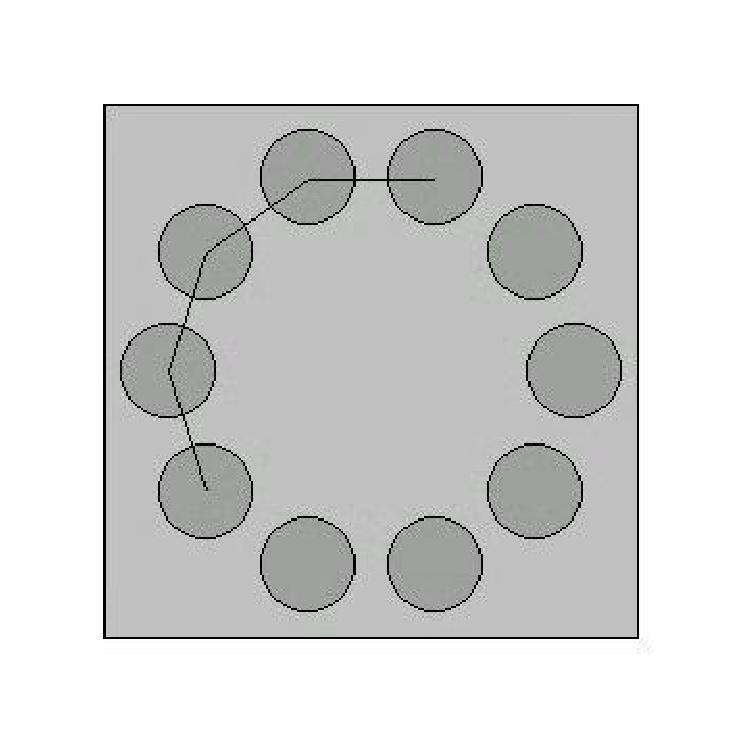
\includegraphics[angle=0,scale=0.3]{heatavi1.eps} & 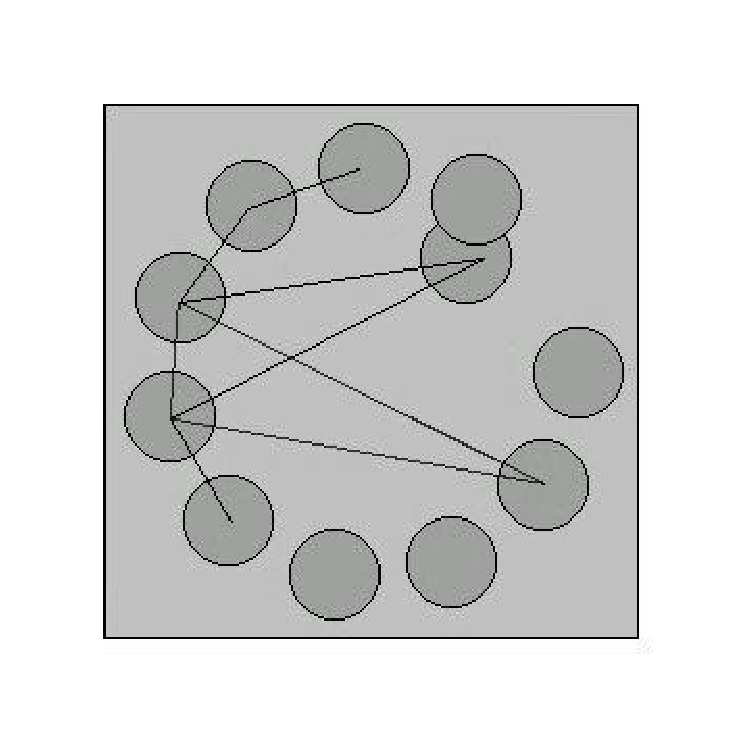
\includegraphics[angle=0,scale=0.3]{heatavi2.eps} &
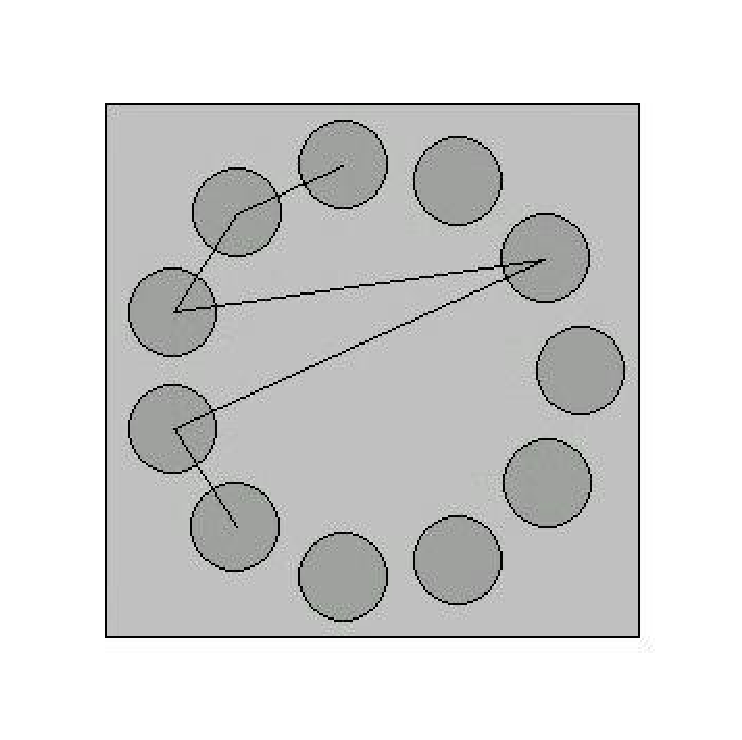
\includegraphics[angle=0,scale=0.3]{heatavi3.eps} \\
\end{tabular}
\caption{These three figures, from left to right, were captured from OverView when an actor was created. 
The outer square represents a SALSA theater, while the inner circles 
represent SALSA actors. Lines between actors represent SALSA message sending behavior.}
\label{heatExample}
\end{figure}

\emph{Please note that OverView requires Java 1.5 to compile and run.}

\section{Using OverView with SALSA Programs}
To visualize SALSA programs, we instrument SALSA (that is, insert event-sending behavior) into SALSA itself; in this way, any executed SALSA program may be visualized, if desired, without any additional configuration.

The easiest way to use OverView to visualize SALSA programs is to download the latest OverView-instrumented SALSA binary, which can be found at:
\begin{description}
  \item {\tt http://wcl.cs.rpi.edu/overview/}
\end{description}

You should download {\tt overview<version>.jar} and {\tt salsa<version>i.jar}, and place them in a convenient location. When executing your SALSA application, simply ensure that both JAR files are in your Java classpath (by either using the {/tt CLASSPATH} environment variable, or by using the {\tt -cp} command line switch).

\emph{If you wish to compile OverView and SALSA from source and instrument SALSA yourself, please see the respective documentations for OverView and SALSA.}

To run OverView and visualize your SALSA application, you must keep in mind that {\tt event sinks} must be started before {\tt event sources}; in practical terms, this means that the OverView visualization must be running before you start your SALSA program.

To do so is relatively simple: you will need an {\it OverView Daemon} (OVD) to collect and forward events, and an {\it OverView Presenter} (OVP) to display the visualization.

\begin{description}
  \item{\tt java overview.ovd.OverViewDaemon}
  \item{\tt java overview.ovp.OverViewPresenter <host:port of OVD>}
\end{description}

\emph{If you are running OVP and OVD on the same machine, OVD's host:port will generally be {\tt localhost:6060}.}

After OverView is running, you may start your SALSA theaters, name servers, and so on. Merely note that every SALSA program that is run (including theaters!) must have the command line switch {\tt -DovHost=<host:port of OVD>} to enable event sending, and to tell SALSA where to send events.

\emph{If you wish to use the instrumented version of SALSA without OverView, simply don't specify {\tt -DovHost}! SALSA programs will then run as usual, without trying to send events.}
 
You can test OverView and SALSA with the following SALSA example:
{\sloppy
\begin{description}
  \item{\tt java -DovHost=<host:port of OVD> examples.fibonacci.Fibonacci 6}
\end{description}
}

You should begin to see a visualization of the sequence of Fibonacci numbers being calculated recursively, using SALSA actors.

\chapter{History of SALSA}
SALSA has been developed since 1998 by Carlos A. Varela, who was a Ph.D. student directed by Gul Agha at
University of Illinois at Urbana-Champaign (UIUC). During the UIUC period, Gregory Haik, a student of Gul Agha, 
has contributions to the naming service of the very early SALSA. 
Carlos A. Varela founded the Worldwide Computing Laboratory and continued the development of SALSA
when he became a faculty member at Rensselaer Polytechnic Institute in 2001.
Many of his students have participated in the SALSA project since then,
including Wei-Jen Wang,
Travis Desell, Kaoutar El Maghraoui, Jason LaPorte,
Abe Stephens, and Robin Toll.
Abe Stephens and Travis Desell were the major contributors of the early version of SALSA at RPI.
They worked together from 2001 until Abe Stephens graduated. Robin Toll has helped 
the early SALSA compiler during this period of time.
From 2003 to 2004, Travis Desell has committed a thoroughly change on the early SALSA, which then became the
foundation of the current version of SALSA. Advanced features such as message properties, 
name tokens, and join block continuations were introduced at that time. 
Wei-Jen Wang and Kaoutar El Maghraoui joined the SALSA project since 2003.
Kaoutar El Maghraoui has major contributions to the development of the communication layer of 
the latest SALSA.
Wei-Jen Wang has been a major developer since 2004. 
He made another major change on SALSA in 2004 and released it in 2005. 
He introduced actor garbage collection,
fault-tolerance communication using persistent sockets and messages, 
actor name deletion support for naming services, and passing-by-value message delivery.      
Jason LaPorte joined the SALSA project in 2006. His contributions relate to  
the interface between SALSA and the OverView project.   

\chapter{SALSA Grammar}\label{GRAMMAR}{
The SALSA grammar is listed as follows:
%begin{latexonly} 
{\singlespace
\lstinputlisting[frame=no]{code/grammar.txt}
}
%end{latexonly} 
\begin{htmlonly}
 \begin{rawhtml} 
  <table border="1" cellpadding="2" cellspacing="0" style="border-collapse: collapse" bordercolor="#111111" id="AutoNumber1">
   <tr><td><pre>
  \end{rawhtml} 
\input{htmlcode/grammar.txt}
 \begin{rawhtml} 
   </pre></td></tr>
  </table>
\end{rawhtml} 
\end{htmlonly}

}

 
\end{document}
